\documentclass{article}
\usepackage{tikz}

\usetikzlibrary{arrows,decorations.markings}

\title{Computer Organization and Architecture}
\author{Conrad A. Mearns}

\begin{document}

\maketitle

\noindent
\Large Turing Machines
\normalsize
\begin{enumerate}
  \item {Turing's Thesis: Every computation can be represented with a Turing Machine.}
  \item {Turing Machine: A mathematical model of a device that can preform any computation.}
  \item {Universal Turing Machine: A machine to implement any and all Turing Machines.}
\end{enumerate}

Beyond models, real world constraints include time, financial cost, power, security, thermal dissapation, space, etc.\\

\noindent
\Large Bits, Data Types, and Operators\\
\normalsize
\indent
The electro-magnetic field is not digital, yet all of modern computing is represented digitally. To compromise, 0 is a representation of the absence of voltage and 1 is a representation of the presence of voltage.

\centering
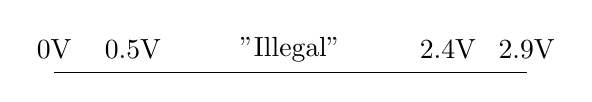
\begin{tikzpicture}
  \node (a) at (0,1) {0V};
  \node (b) at (1,1) {0.5V};
  \node (c) at (5,1) {2.4V};
  \node (d) at (6,1) {2.9V};
  \node (b) at (3,1) {"Illegal"};
  \draw (0,.7) -- (6,.7);
\end{tikzpicture}
\raggedright

\noindent
\Large
Signed Binary Arithmetic\\
\normalsize
\indent
Binary, without the addition of extra mathematical symbols, can only represent positive whole integers. Signed numbers like $-5$ require a formal system of representation in order to be used. A binary number can represent $2^n$ values for $n$ bits. The objective of signed numbers is to partition half of those values for negative number representation ($-2^{n-1}-1 \to -1$) and the other half to positive numbers ($1 \to 2^{n-1}$) while leaving zero and potentially one other number available.

\begin{enumerate}
  \item {
  Sign-Magnitude\\
  The most significant bit is 0 for positive values and 1 for negative values.\\
  $00101 = 5$ and $10101 = -5$
  }
  \item {
  One's Complement\\
  All bits are inversed to represent negative numbers. Like Sign-Magnitude, the most significant bit will tell you whether a number is positive or negative.\\
  $00101 = 5$ and $11010 = -5$
  }
  \item {
  Two's Complement (currently in use)\\
  For each positive number $A$, it's negative number ($B$) satisfies the equation $A + B = 0$ when the final carried bit is dropped. To get this number, take the One's Complement of $A$ and add 1.
  $00101 = 5$ and the One's Complement is $11010$. So the Two's Complement is $11011$. As proof, $00101 + 11011 = 100000$ but the last carried one is dropped, leaving $00000$.
  }
\end{enumerate}

\noindent
\Large
Arithmetic and Logical Operations\\
\normalsize
\noindent
Arithmetic operations
\begin{enumerate}
  \item {Addition\\Just addition, regardless if signed or not. Ignore the final carry-out.}
  \item {Subtraction\\First negate the second operand ($5 \to -5 for example$), then use addition.}
  \item {Sign Extension\\To add numbers, they must have the same number of bits. This is because of signed numbers, and storage.}
\end{enumerate}

\noindent
Overflow occurs when
\begin{enumerate}
  \item Signs of the operands are the same
  \item The sign of the sum is different
\end{enumerate}
\noindent
The issue can be tested for by examining the most significant bit's sign between the operands and the result.

\noindent
Logical operations
\begin{enumerate}
  \item {AND\\The result is true if and only if both operands are true.\\Useful for clearing bits, a mask of 1's signify keep.}
  \item {OR\\The result is true if either operand is true.\\Useful for setting bits. 1's in the second operand copy to the result.}
  \item {NOT\\The result is true if and only if the operand is false.}
\end{enumerate}
\noindent
Each operation is executed on each bit individually.

\noindent
\Large
Fractions, Floating, and Fixed-Point Values\\
\normalsize
\indent
A "binary" point is abstractly added to the value. To the left of the point, each bit is worth is $2^{-n}$ where n is the place left of the point. For example, $101.11$.

For large numbers, we use scientific notation. $Sign * (Fraction * 2^{Exponent})$
IEEE 754 Floating Point Standard for 32-bits signifies 1 bit for sign, 8 bits for the exponenant, and 23 bits for the fraction.
$1 01111110 10000000000000000000000 = -1.5*2^{???}$

\noindent
\Large
Other Date Types
\normalsize
\indent
\begin{enumerate}
  \item Single characters use ASCII to map 128 characters to 7-bit code.
  \item Text strings are sequences of characters often with a NULL to terminate. No hardware support.
  \item Images are arrays of images. Often has hardware support.
  \item Sound is a sequence of fixed-point numbers.
\end{enumerate}

\end{document}
